\begin{frame}{Introduction and history }
 \begin{columns}
     \begin{column}{0.6\textwidth}
          \begin{block}{}
	
    \begin{itemize}
    \item 
    \textbf{Computational model} introduced by John Von Neumann and Stanislaw Ulam in the 1940s
    \item 
    It consists of a \textbf{grid of cells}, each in one of a finite number of \textbf{states} that change in \textbf{discrete time} steps according to a \textbf{fixed rule} based on cell's \textbf{neighbourhood}
        \item \textbf{Famous examples:}  Wolfram's elementary cellular automata (1980s), Conway's game of life (1970s)...
    \end{itemize}
  \end{block}
     \end{column}
    \column{0.4\textwidth}
        \centering
        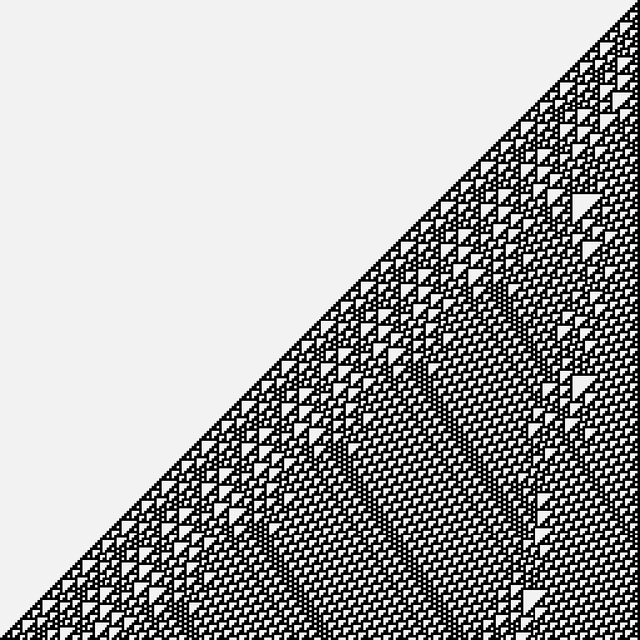
\includegraphics[height=0.4\textheight]{Sample_run_of_Rule_110.png}
        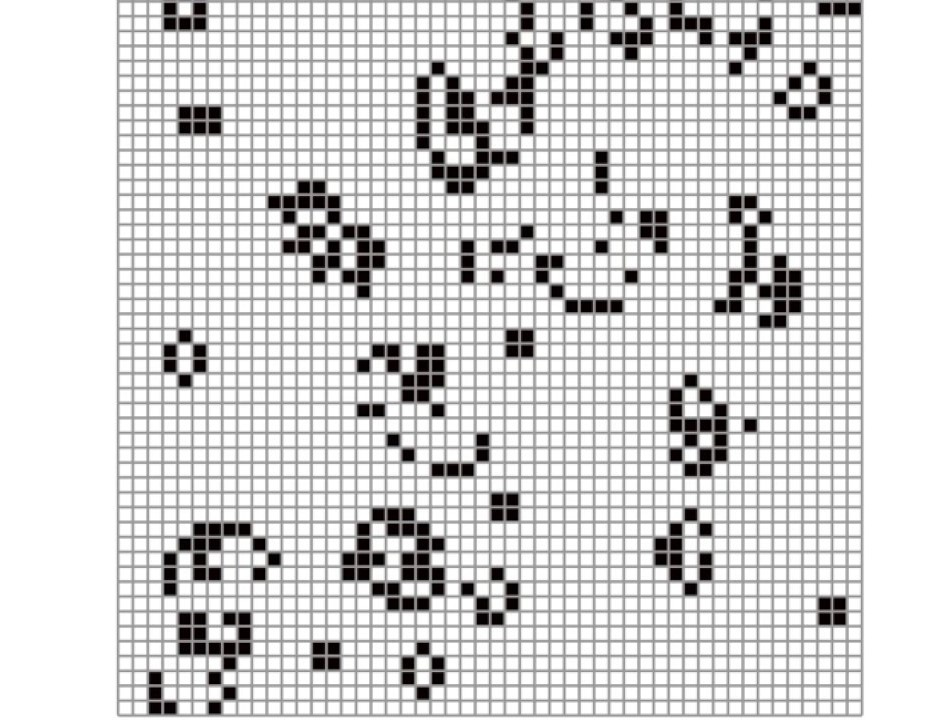
\includegraphics[height=0.4\textheight]{conwaygame.jpg}
 \end{columns}
\end{frame}


\begin{frame}{Core Idea}

\begin{columns}
    \begin{column}{0.8\textwidth}
                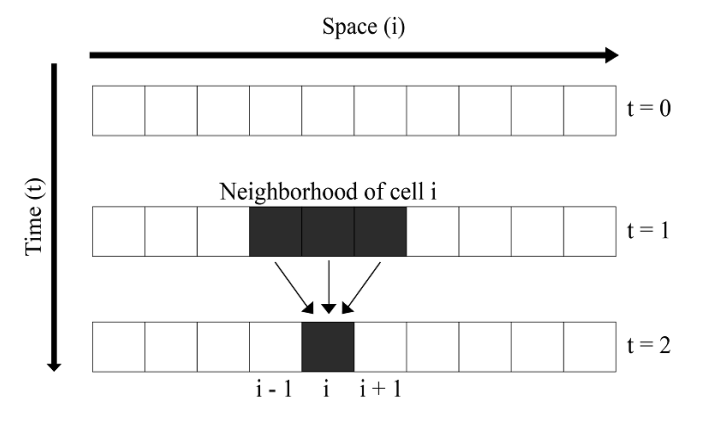
\includegraphics[width = 1.0\textwidth]{slike/intro.png}

    \end{column}
    \begin{column}{0.5\textwidth}
                    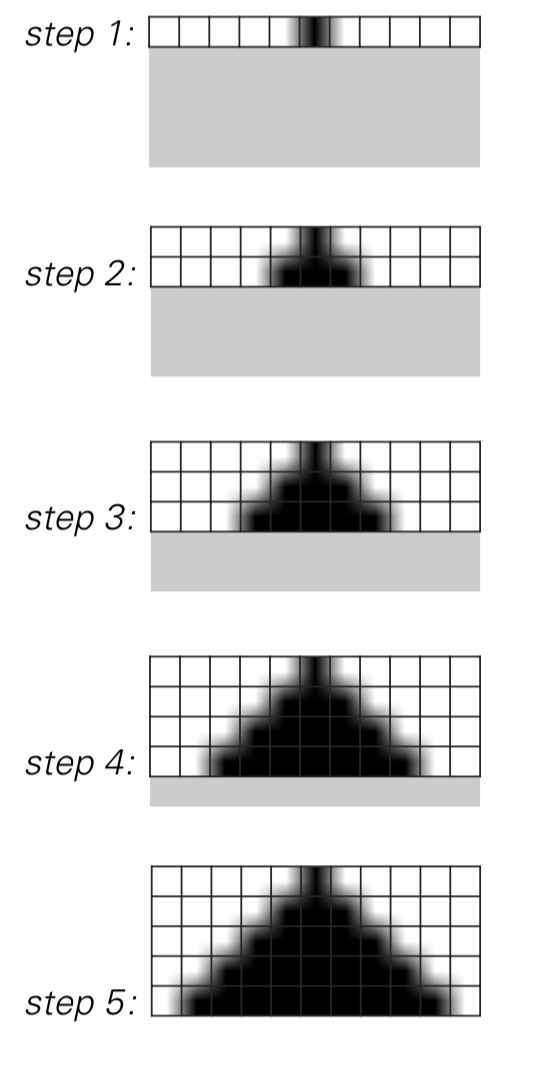
\includegraphics[width = 0.6\textwidth]{timeprogression.jpg}

    \end{column}
\end{columns}

\end{frame}

\begin{frame}{Motivating example (Rule 90)}
  \begin{exampleblock}{}
      \centering
    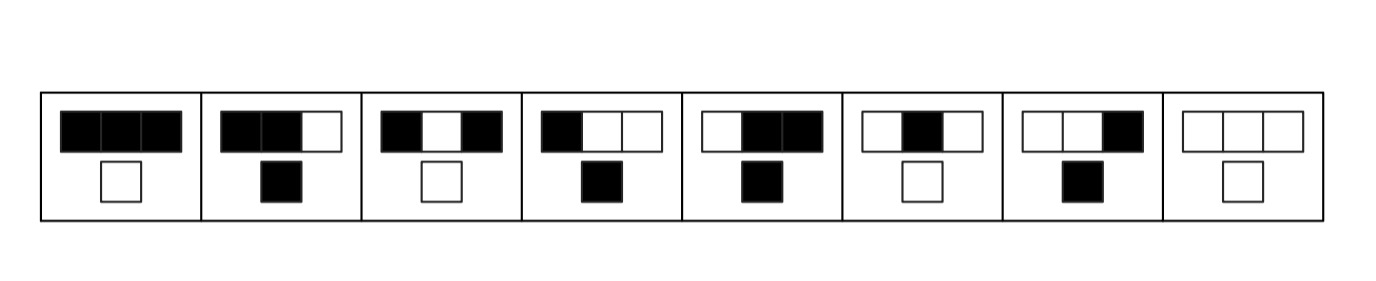
\includegraphics[width = 0.8\textwidth]{Rule90.jpeg}
  \end{exampleblock}
  \begin{block}{Cellular State Space}
  Two states: black - 1 (live), white  - 0 (dead)
  \end{block}
  \begin{block}{Update Rule}
    At each time step: XOR of two neighbouring values
  \end{block}
\end{frame}

\begin{frame}{Motivating example (Rule 90)}
\begin{columns}
    \begin{column}{0.5\textwidth}
                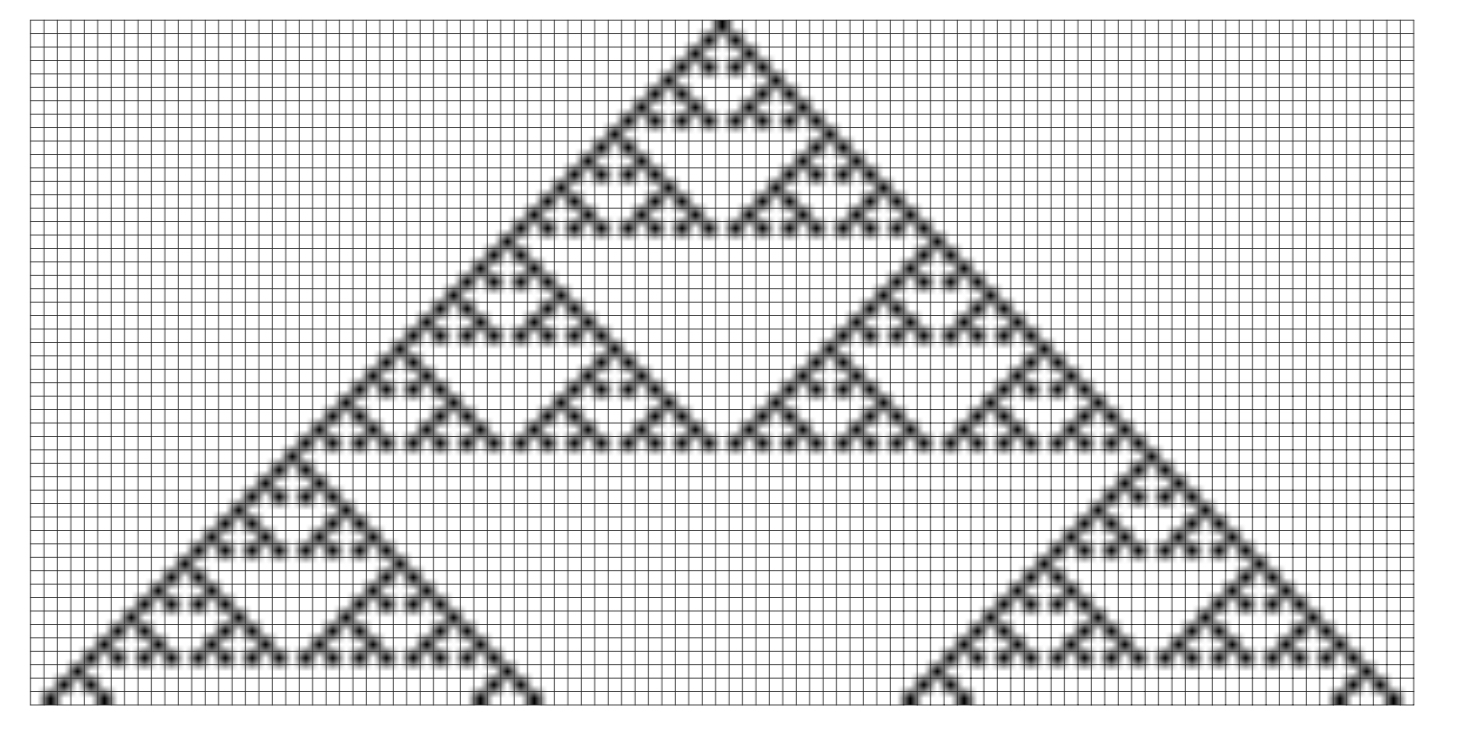
\includegraphics[width = 1.0\textwidth]{slike/rule90evolution.jpeg}
                Sierpinski triangle (from a single live cell)
    \end{column}
    \begin{column}{0.5\textwidth}
                    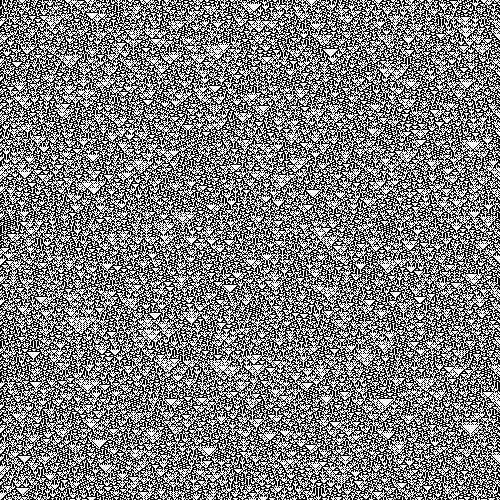
\includegraphics[width = 0.9\textwidth]{randomrule90.png}
                    Time space diagram (random initial conditions)
    \end{column}
\end{columns}

\end{frame}

\begin{frame}{Notations and definition}
	  \begin{itemize}
	  \item \textbf{Discrete cellular state space} $\mathcal{L}$: $n$-dimensional lattice of cells of possibly different shapes (usually homogenous)
	  \item \textbf{Local value space} $\Sigma$: Each cell is in exactly \textbf{one state} $$\sigma_{\vec{i}\in \mathcal{L}}(t) \in \Sigma\equiv \{0,1,2,\dots,k-1 \}$$ The number of possible states is  $k =|\Sigma|$. 
   \item \textbf{Boundary conditions} (when the simulation is run on finite sets)
	  \item \textbf{Dynamical rule} $\phi: \Sigma^n \to \Sigma$, where $n$ specifies the number of cells of the neighbourhood $\mathcal{N}\{\vec{i}\}$ about cell $\vec{i}$. Transition rule is written as
        $$\sigma_{\vec{i}}(t+1) = \phi(\sigma_{\vec{j}}(t)\in \mathcal{N}\{\vec{i}\})$$ 
	  \end{itemize}
	
	

\end{frame}


\begin{frame}{One-dimensional example}
 
  \begin{columns}
	\begin{column}{0.5\textwidth}
	  \begin{itemize}
	  \item One-dimensional lattice
	  \item $\Sigma =\{0,1\}, k = 2$
	  \item No boundary conditions
        \item Neighbourhood of a cell having radius $r=1$ (to the left and right of cell) 
        \item Dynamical rule represented with a diagram for $k^{2r+1} = 8$ neighbourhood states.
        \item $k^{k^{2r+1}}=2^8= 256$ possible different rules 
	  \end{itemize}
   	  
	\end{column}
	\begin{column}{0.7\textwidth}
 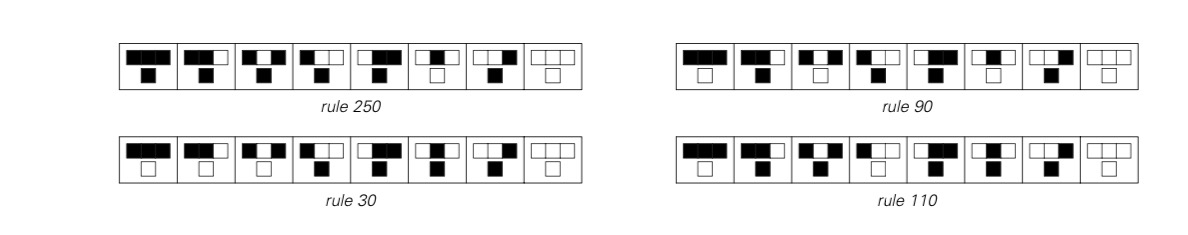
\includegraphics[height=0.18\textheight]{slike/rules.jpeg}
        \centering
        
        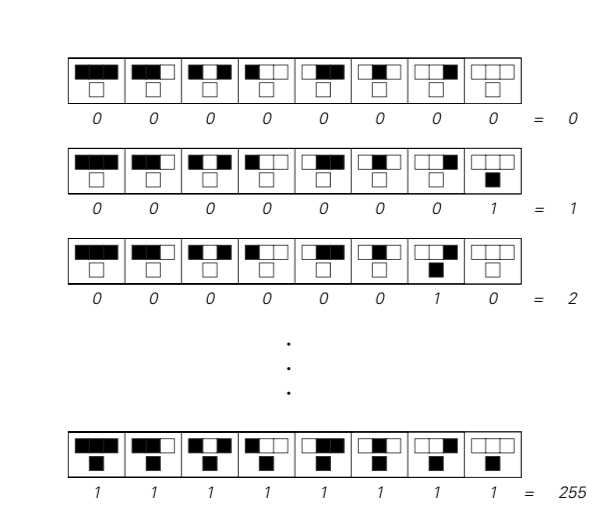
\includegraphics[height=0.6\textheight]{slike/PossibleRules.jpeg}
        \end{column}
    \end{columns}
\end{frame}
